\documentclass[english,,man,floatsintext]{apa6}
\usepackage{lmodern}
\usepackage{amssymb,amsmath}
\usepackage{ifxetex,ifluatex}
\usepackage{fixltx2e} % provides \textsubscript
\ifnum 0\ifxetex 1\fi\ifluatex 1\fi=0 % if pdftex
  \usepackage[T1]{fontenc}
  \usepackage[utf8]{inputenc}
\else % if luatex or xelatex
  \ifxetex
    \usepackage{mathspec}
  \else
    \usepackage{fontspec}
  \fi
  \defaultfontfeatures{Ligatures=TeX,Scale=MatchLowercase}
\fi
% use upquote if available, for straight quotes in verbatim environments
\IfFileExists{upquote.sty}{\usepackage{upquote}}{}
% use microtype if available
\IfFileExists{microtype.sty}{%
\usepackage{microtype}
\UseMicrotypeSet[protrusion]{basicmath} % disable protrusion for tt fonts
}{}
\usepackage{hyperref}
\hypersetup{unicode=true,
            pdftitle={Psychological Science needs a standard practice of reporting reliabilty},
            pdfauthor={Sam Parsons, Anne-Wil Kruijt, \& Elaine Fox},
            pdfkeywords={reliability, estimating and reporting, cognitive-behavioural tasks, psychometrics},
            pdfborder={0 0 0},
            breaklinks=true}
\urlstyle{same}  % don't use monospace font for urls
\ifnum 0\ifxetex 1\fi\ifluatex 1\fi=0 % if pdftex
  \usepackage[shorthands=off,main=english]{babel}
\else
  \usepackage{polyglossia}
  \setmainlanguage[]{english}
\fi
\usepackage{color}
\usepackage{fancyvrb}
\newcommand{\VerbBar}{|}
\newcommand{\VERB}{\Verb[commandchars=\\\{\}]}
\DefineVerbatimEnvironment{Highlighting}{Verbatim}{commandchars=\\\{\}}
% Add ',fontsize=\small' for more characters per line
\usepackage{framed}
\definecolor{shadecolor}{RGB}{248,248,248}
\newenvironment{Shaded}{\begin{snugshade}}{\end{snugshade}}
\newcommand{\AlertTok}[1]{\textcolor[rgb]{0.94,0.16,0.16}{#1}}
\newcommand{\AnnotationTok}[1]{\textcolor[rgb]{0.56,0.35,0.01}{\textbf{\textit{#1}}}}
\newcommand{\AttributeTok}[1]{\textcolor[rgb]{0.77,0.63,0.00}{#1}}
\newcommand{\BaseNTok}[1]{\textcolor[rgb]{0.00,0.00,0.81}{#1}}
\newcommand{\BuiltInTok}[1]{#1}
\newcommand{\CharTok}[1]{\textcolor[rgb]{0.31,0.60,0.02}{#1}}
\newcommand{\CommentTok}[1]{\textcolor[rgb]{0.56,0.35,0.01}{\textit{#1}}}
\newcommand{\CommentVarTok}[1]{\textcolor[rgb]{0.56,0.35,0.01}{\textbf{\textit{#1}}}}
\newcommand{\ConstantTok}[1]{\textcolor[rgb]{0.00,0.00,0.00}{#1}}
\newcommand{\ControlFlowTok}[1]{\textcolor[rgb]{0.13,0.29,0.53}{\textbf{#1}}}
\newcommand{\DataTypeTok}[1]{\textcolor[rgb]{0.13,0.29,0.53}{#1}}
\newcommand{\DecValTok}[1]{\textcolor[rgb]{0.00,0.00,0.81}{#1}}
\newcommand{\DocumentationTok}[1]{\textcolor[rgb]{0.56,0.35,0.01}{\textbf{\textit{#1}}}}
\newcommand{\ErrorTok}[1]{\textcolor[rgb]{0.64,0.00,0.00}{\textbf{#1}}}
\newcommand{\ExtensionTok}[1]{#1}
\newcommand{\FloatTok}[1]{\textcolor[rgb]{0.00,0.00,0.81}{#1}}
\newcommand{\FunctionTok}[1]{\textcolor[rgb]{0.00,0.00,0.00}{#1}}
\newcommand{\ImportTok}[1]{#1}
\newcommand{\InformationTok}[1]{\textcolor[rgb]{0.56,0.35,0.01}{\textbf{\textit{#1}}}}
\newcommand{\KeywordTok}[1]{\textcolor[rgb]{0.13,0.29,0.53}{\textbf{#1}}}
\newcommand{\NormalTok}[1]{#1}
\newcommand{\OperatorTok}[1]{\textcolor[rgb]{0.81,0.36,0.00}{\textbf{#1}}}
\newcommand{\OtherTok}[1]{\textcolor[rgb]{0.56,0.35,0.01}{#1}}
\newcommand{\PreprocessorTok}[1]{\textcolor[rgb]{0.56,0.35,0.01}{\textit{#1}}}
\newcommand{\RegionMarkerTok}[1]{#1}
\newcommand{\SpecialCharTok}[1]{\textcolor[rgb]{0.00,0.00,0.00}{#1}}
\newcommand{\SpecialStringTok}[1]{\textcolor[rgb]{0.31,0.60,0.02}{#1}}
\newcommand{\StringTok}[1]{\textcolor[rgb]{0.31,0.60,0.02}{#1}}
\newcommand{\VariableTok}[1]{\textcolor[rgb]{0.00,0.00,0.00}{#1}}
\newcommand{\VerbatimStringTok}[1]{\textcolor[rgb]{0.31,0.60,0.02}{#1}}
\newcommand{\WarningTok}[1]{\textcolor[rgb]{0.56,0.35,0.01}{\textbf{\textit{#1}}}}
\usepackage{graphicx,grffile}
\makeatletter
\def\maxwidth{\ifdim\Gin@nat@width>\linewidth\linewidth\else\Gin@nat@width\fi}
\def\maxheight{\ifdim\Gin@nat@height>\textheight\textheight\else\Gin@nat@height\fi}
\makeatother
% Scale images if necessary, so that they will not overflow the page
% margins by default, and it is still possible to overwrite the defaults
% using explicit options in \includegraphics[width, height, ...]{}
\setkeys{Gin}{width=\maxwidth,height=\maxheight,keepaspectratio}
\IfFileExists{parskip.sty}{%
\usepackage{parskip}
}{% else
\setlength{\parindent}{0pt}
\setlength{\parskip}{6pt plus 2pt minus 1pt}
}
\setlength{\emergencystretch}{3em}  % prevent overfull lines
\providecommand{\tightlist}{%
  \setlength{\itemsep}{0pt}\setlength{\parskip}{0pt}}
\setcounter{secnumdepth}{0}
% Redefines (sub)paragraphs to behave more like sections
\ifx\paragraph\undefined\else
\let\oldparagraph\paragraph
\renewcommand{\paragraph}[1]{\oldparagraph{#1}\mbox{}}
\fi
\ifx\subparagraph\undefined\else
\let\oldsubparagraph\subparagraph
\renewcommand{\subparagraph}[1]{\oldsubparagraph{#1}\mbox{}}
\fi

%%% Use protect on footnotes to avoid problems with footnotes in titles
\let\rmarkdownfootnote\footnote%
\def\footnote{\protect\rmarkdownfootnote}


  \title{Psychological Science needs a standard practice of reporting reliabilty}
    \author{Sam Parsons\textsuperscript{1}, Anne-Wil Kruijt\textsuperscript{2}, \& Elaine Fox\textsuperscript{1}}
    \date{}
  
\shorttitle{Reporting reliability as standard}
\affiliation{
\vspace{0.5cm}
\textsuperscript{1} Department of Experimental Psychology, University of Oxford\\\textsuperscript{2} Department of Psychology, Stockholm University}
\keywords{reliability, estimating and reporting, cognitive-behavioural tasks, psychometrics\newline\indent Word count: 9178}
\usepackage{csquotes}
\usepackage{upgreek}
\captionsetup{font=singlespacing,justification=justified}

\usepackage{longtable}
\usepackage{lscape}
\usepackage{multirow}
\usepackage{tabularx}
\usepackage[flushleft]{threeparttable}
\usepackage{threeparttablex}

\newenvironment{lltable}{\begin{landscape}\begin{center}\begin{ThreePartTable}}{\end{ThreePartTable}\end{center}\end{landscape}}

\makeatletter
\newcommand\LastLTentrywidth{1em}
\newlength\longtablewidth
\setlength{\longtablewidth}{1in}
\newcommand{\getlongtablewidth}{\begingroup \ifcsname LT@\roman{LT@tables}\endcsname \global\longtablewidth=0pt \renewcommand{\LT@entry}[2]{\global\advance\longtablewidth by ##2\relax\gdef\LastLTentrywidth{##2}}\@nameuse{LT@\roman{LT@tables}} \fi \endgroup}
\usepackage{float}
\usepackage{caption}
\floatplacement{figure}{H}
\raggedbottom

\authornote{Author's contributions: SP conceived and wrote the manuscript. Throughout, AW-K provided crucial conceptual and theoretical feedback. All authors provided critical feedback to develop the final manuscript, for which all authors agreed upon.

We would like to thank Craig Hedge for making data open and available. We would also like to thank all those that provided feedback on the preprint version of this paper (\url{https://psyarxiv.com/6ka9z}). The comments, critical feedback, and articles shared have helped to develop of this manuscript. In alphabetical order (apologies to anybody missed), we thank; James Bartlett, Paul Christiansen, Oliver Clarke, Andrew Jones, Michael Kane, Jesse Kaye, Kevin King, Mike Lawrence, Marcus Munafo, Cliodhna O'Connor, Oscar Olvera, Oliver Robinson, Guillaume Rousselet, and Bruno Zumbo.

The data and code used to create this manuscript can be found at \url{https://osf.io/9jp65/}

This is version 3: 6/2019

Correspondence concerning this article should be addressed to Sam Parsons, Department of Experimental Psychology, University of Oxford. E-mail: \href{mailto:sam.parsons@psy.ox.ac.uk}{\nolinkurl{sam.parsons@psy.ox.ac.uk}}}
\note{\clearpage}
\abstract{
Psychological science relies on behavioural measures to assess cognitive processing; however, the field has not yet developed a tradition of routinely examining the reliability of these behavioural measures. Reliable measures are essential to draw robust inferences from statistical analyses, while subpar reliability has severe implications for the measures' validity and interpretation. Without examining and reporting the reliability of cognitive behavioural measurements, it is near impossible to ascertain whether results are robust or have arisen largely from measurement error. In this paper we propose that researchers adopt a standard practice of estimating and reporting the reliability of behavioural assessments. We illustrate this proposal using an example from experimental psychopathology, the dot-probe task; although we argue that reporting reliability is relevant across fields (e.g.~social cognition and cognitive psychology). We explore several implications of low measurement reliability, and the detrimental impact that failure to assess measurement reliability has on interpretability and comparison of results and therefore research quality. We argue that the field needs to a) report measurement reliability as routine practice so that we can b) develop more reliable assessment tools. To provide some guidance on estimating and reporting reliability, we describe bootstrapped split half estimation and IntraClass Correlation Coefficient procedures to estimate internal consistency and test-retest reliability, respectively. For future researchers to build upon current results it is imperative that all researchers provide sufficient psychometric information to estimate the accuracy of inferences and inform further development of cognitive behavioural assessments.



}

\begin{document}
\maketitle

\setlength{\abovedisplayskip}{-20pt}
\setlength{\belowdisplayskip}{3pt}
\setlength{\abovedisplayshortskip}{-30pt}
\setlength{\belowdisplayshortskip}{3pt}

\begin{quote}
In essence, it is as if I-P {[}Information Processing{]} researchers have been granted psychometric free rein that would probably never be extended to researchers using other measures, such as questionnaires.
\end{quote}

\begin{quote}
\hfill --- Vasey, Dalgleish, \& Silverman (2003)
\end{quote}

The central argument of this paper is that psychological science stands to benefit greatly from adopting a standard practice of estimating and reporting the reliability of behavioural assessments in psychological science. Behavioural assessments are commonly used in psychological science to examine cognitive processing, yet they rarely receive sufficient psychometric scrutiny. This paper aims to outline how reporting basic psychometrics will improve our current research practices in psychological science. We use the experimental psychopathology field as an example of where adoption of these reporting practices will be of particular value; although these recommendations apply broadly to any approach that relies on behavioural assessment of cognitive functions. Sixteen years ago, Vasey, Dalgleish, and Silverman (2003, p. 84) published the quote above and we echo their concern. Our impression is that while pockets of information-processing researchers have begun to appreciate the importance of measure reliability, little has changed in practice. We hope that this paper helps to spark the small changes required to achieve a simple but conceivably significant improvement to the research quality and practice in the experimental psychopathology field, as well as psychological science more generally.

All measures, and therefore all analyses, are \enquote{contaminated} by measurement error. Reliability estimates provide researchers with an indication of the degree of contamination, enabling better judgments about the implications of their analyses. Various authors have stressed the importance of measurement reliability, for example; \enquote{Interpreting the size of observed effects requires an assessment of the reliability of the scores} (Wilkinson, 1999, p. 596), and \enquote{Researchers should calibrate their confidence in their experimental results as a function of the amount of random measurement error contaminating the scores of the dependent variable.} (LeBel \& Paunonen, 2011; also see Cooper, Gonthier, Barch, \& Braver, 2017; Hedge, Powell, \& Sumner, 2018). Psychometric consideration is usually afforded to self-report measures; we argue that measurement is equally important for cognitive-behavioural measures.

Reliability is not an inherent property of a task. Therefore, neither the term \enquote{reliability} nor the obtained estimates should be used to refer to the task itself; reliability refers to the measurement obtained and not to the task used to obtain it. A number of authors have made this same point (for a few examples, see Appelbaum et al., 2018; Cooper et al., 2017; Hedge et al., 2018; LeBel \& Paunonen, 2011; and Wilkinson, 1999). Nonetheless, it warrants emphasising that reliability is estimated from the scores obtained with a particular task from a particular sample under specific circumstances (we use \enquote{measure} and \enquote{measurement} throughout this paper to refer to the measurements obtained, and not the task used). We cannot infer that a reliability estimate obtained for a certain measure in one sample, or test manual, will generalise to other study samples using the same task. This has been described as \enquote{reliability induction} (Vacha-Haase, Henson, \& Caruso, 2002). Thus, researchers cannot assume a level of reliability in their measures without examination of the psychometric properties obtained in that particular study sample. It is, therefore, not surprising that psychological research holds an expectation to report reliability and validity evidence for self-report questionnaires (e.g.~APA reporting guidelines, Appelbaum et al., 2018). However, recent evidence has demonstrated severe underreporting of scale validity and reliability evidence (Flake, Pek, \& Hehman, 2017), as well as crucial validity issues -- such as lack of measurement invariance -- that remain hidden due to this underreporting (Hussey \& Hughes, 2018).

The current paper is specifically concerned with the psychometrics of cognitive behavioural tasks, which are equally influenced by the reliability and validity issues raised by Flake et al.~(2017) and Hussey \& Hughes (2018). We argue that careful interpretation of results requires a practice of estimating and reporting measurement reliability to accompany the analyses of task measurements' outcomes. Unfortunately, appraising the psychometrics of these measures is the exception rather than the rule (Gawronski, Deutsch, \& Banse, 2011; Vasey et al., 2003). Underreporting the psychometric properties of task measurements may be more problematic as these tasks are often adapted depending on the nature of the research question, for example by modifying the task stimuli (as opposed to the common practice with respect to questionnaire measures for which the format tends be standardised and study-specific alterations may be frowned upon).

Without the standard practice of reporting the psychometrics of our measures it is; a) difficult to determine how common or widespread reliability problems are with cognitive behavioural measures; b) near impossible to assess the validity of previous research using these measures; c) challenging to verify if changes to our measures result in improved reliability and/or validity; and d) difficult, if not impossible, to compare effect sizes between studies. Therefore, the absence of simple reliability estimates undermines confidence in study results and impedes progress. Cumulative science rests on the foundations of our measurements, and building a sound research base will only be possible when researchers report measurement psychometrics for each and every study. Therefore, we recommend that researchers estimate and report measurement reliability as standard practice, whether using questionnaire or cognitive behavioural measures.

By the end of this paper, we aim that readers a) are made aware of the importance of routine reporting of measurement reliability, and b) have several tools to begin estimating the reliability of their own tasks. This paper is split into two parts. In the first part we discuss the implications of measurement reliability on results, which are often hidden due to lack of reporting. In this, we discuss implications of unreliable cognitive behavioural measures and argue that they are intensified by the lack of a standard practice to assess and report estimates of measurement reliability. We go on to discuss an example from our own field of experimental psychopathology to highlight some of these issues more concretely. In the second part of this paper, we provide more practical guidance on implementing the routine reporting of internal consistency and test-retest reliability estimates. We also provide example code to obtain reliability estimates, using simple commands in the R environment\footnote{We used R (Version 3.5.2; R Core Team, 2018) and the R-packages \emph{dplyr} (Version 0.8.0.1; Wickham et al., 2019), \emph{forcats} (Version 0.4.0; Wickham, 2019a), \emph{formatR} (Version 1.6; Xie, 2019), \emph{ggplot2} (Version 3.1.1; Wickham, 2016), \emph{koRpus} (Version 0.11.5; Michalke, 2018a, 2019), \emph{koRpus.lang.en} (Version 0.1.3; Michalke, 2019), \emph{papaja} (Version 0.1.0.9842; Aust \& Barth, 2018), \emph{psych} (Version 1.8.12; Revelle, 2018), \emph{purrr} (Version 0.3.2; Henry \& Wickham, 2019), \emph{pwr} (Version 1.2.2; Champely, 2018), \emph{readr} (Version 1.3.1; Wickham, Hester, \& Francois, 2018), \emph{splithalf} (Version 0.5.2; Parsons, 2017), \emph{stringr} (Version 1.4.0; Wickham, 2019b), \emph{sylly} (Version 0.1.5; Michalke, 2018b), \emph{tibble} (Version 2.1.1; Müller \& Wickham, 2019), \emph{tidyr} (Version 0.8.3; Wickham \& Henry, 2019), \emph{tidyverse} (Version 1.2.1; Wickham, 2017), \emph{tufte} (Version 0.5; Xie \& Allaire, 2019), and \emph{wordcountaddin} (Version 0.3.0.9000; Marwick, 2019) for all analyses and figures, and to generate this document.} to analyse publicly available Stroop task data (Hedge et al., 2018). Finally, we make suggestions on the transparent and complete reporting of reliability estimates.

\hypertarget{on-the-importance-of-measurement-reliability}{%
\section{On the importance of measurement reliability}\label{on-the-importance-of-measurement-reliability}}

In this section we highlight two important aspects of research for which measurement reliability plays an important role; statistical power, and comparisons of results. To evaluate the impact on both, reliability estimates must be reported as standard.

\hypertarget{reliability-and-statistical-power}{%
\subsection{Reliability and statistical power}\label{reliability-and-statistical-power}}

Low statistical power is an ongoing problem in psychological science (e.g.~Button, Lewis, Penton-Voak, \& Munafò, 2013; Morey \& Lakens, 2016). Statistical power is the probability of observing a statistically significant effect for a given alpha (typically .05), a specified sample size, and a (non-zero) population effect. An often-overlooked impact of low power is that, on top of a low probability of observing effects that do exist (a high probability of committing a type 2 error), any observed statistically significant effects are more likely to be false positives (Ioannidis, 2005; Ioannidis, Tarone, \& McLaughlin, 2011). Overlooking the influence of measurement reliability on statistical power may result in an unknowable influence on the precision of statistical tests. Here, we explore the relationship between statistical power and reliability under two research designs; group-differences, and individual-differences.

\hypertarget{power-reliability-and-group-differences}{%
\subsection{Power, reliability, and group-differences}\label{power-reliability-and-group-differences}}

This section will illustrate how reliability has an indirect functional relationship with statistical power. We use a simple group-differences test for an example here. Statistical power is dependent on both group sizes and measurement variance: lower variance yields higher statistical power. As defined by classical test theory, observed-score variance, or \enquote{total} variance is the sum of \enquote{true-score} variance and \enquote{error} score variance (X = T + E). Power depends on the total variance, i.e.~the sum of true-score and error variance. Measurement reliability, on the other hand, is defined as the proportion of variance attributed to true-score relative to total variance (R = T / T + E). As Zimmerman and Zumbo (2015) demonstrated mathematically, the relationship between reliability and power can be observed when either true-score variance or error variance is held constant and the other is left to vary. By adding true-score or error variance; the total variance increases and we can observe the ensuing relationship between reliability and power. Briefly, when true variance is fixed, increases in error variance result in decreases in reliability and decreases in statistical power. In contrast, fixing error variance and increasing true variance leads to increases in reliability, yet, this is accompanied by the decrease in power.

Visualising these relationships can be helpful to illustrate the conceptual differences between reductions in power due to increasing error variance, versus reduced power due to decreased true variance. Figure 1 presents a conceptual representation of the reliability-power relationship depicting the difference. In both panels, as total variance increases (indicated by the width of the error bars), the observed effect size reduces, as does the statistical power for this difference test. The left panel holds true-score (blue line sections) variance constant, while the right panel holds error variance (red line sections) constant; note the resulting reliability (T / T + E) on the y axis. Consider the impact of increasing total variance in both panels. As total variance increases, the observed effect size \(\frac{mean - 0}{\sqrt{total-variance}}\) is reduced. Consequently, statistical power is also reduced proportionally to the increase in total variance. However, each panel shows a different relationship between reliability and statistical power. In the left panel, despite there being a consistent \enquote{true} difference from zero, increases in measurement error obscures the effect: as error increases, the true effect is \enquote{hidden} by error (if the plot would show the standard deviation, i.e.~the square root of the variance) instead of the variance, the distribution would expand to overlap with the reference value from which point onwards it would yield non-significant results if we'd perform a one-sample t-test even though the \enquote{true} effect size remains unaltered). In the right panel, on the other hand, the true effect size decreases as true variance increases -- thus reducing statistical power (i.e.~one needs larger samples to reliably detect an effect that shows a larger true variance). So, while reliability does not have a direct relationship to statistical power, it does offer useful information to aid our interpretations of results. For instance, we would be better able to gauge whether an observed small effect (and low power) is due to measurement error \enquote{obscuring} the effect, or whether it could be a small but genuine effect.

\begin{figure}
\centering
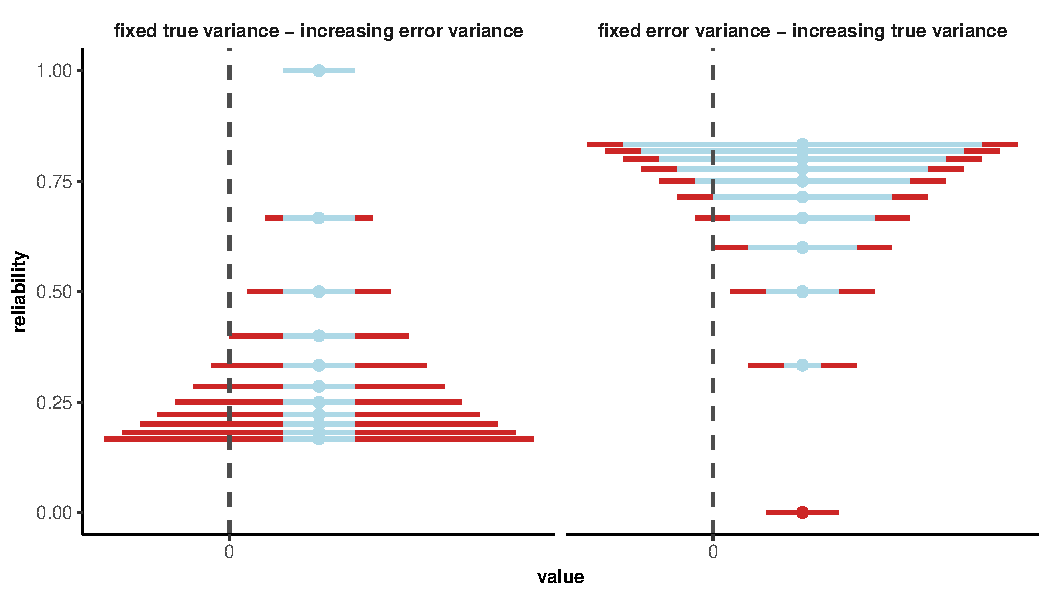
\includegraphics{Parsons_Kruijt_Fox_-_reporting_reliability_files/figure-latex/figureone-1.pdf}
\caption{\label{fig:figureone}Both panels present a comparison between an observed measurement/distribution and a reference value zero. The blue line sections visualise the \enquote{true-score} variance, the red sections the error variance; the total width indicates total variance. The reliability estimate (T / T + E) is indicated on the y axis. Left hand panel: reliability decreases and total variance increases when error variance increases while true-score variance remains constant. Right hand panel: both reliability and total variance decrease when \enquote{true score} variance decreases while error variance remains constant.}
\end{figure}

\hypertarget{power-reliability-and-correlation-correcting-for-reliability}{%
\subsection{Power, reliability, and correlation: correcting for reliability}\label{power-reliability-and-correlation-correcting-for-reliability}}

The reliability of measures constrains the maximum observable correlation between two measures -- we cannot observe a larger association between two variables than the average reliability of those variables. Thus, greater measurement error and reduced between-subjects variance reduces our ability to observe associations between cognitive processes (also see Rouder, Kumar, \& Haaf, 2019). We can estimate this impact beginning with Spearman's (1904) formula to correct for the influence of measurement error on correlational analysis (also known as the attenuation-correction formula);

\begin{align}
r_{true}=\frac{r_{observed}}{\sqrt{r_{xx} \times r_{yy}}}
\end{align}

Reliability estimates are estimates of the autocorrelation (i.e.~r\_xx and r\_yy in the formula above). In other words: the \enquote{true correlation} between the \enquote{true scores} of x and y is the observed correlation divided by the square root of the product of the autocorrelations for both measurements. We can then rearrange Spearman's formula to the following;

\begin{align}
r_{observed}=r_{true} \sqrt{reliability(x) \times reliability ~(y) ~}
\end{align}

Using the re-arranged formula we can calculate the expected power for an observable correlation that has been powered at 80\% to observe a correlation of at least the size of the expected \enquote{true} correlation. To illustrate, we might expect a \enquote{true} correlation of .5 between two measures. If, both measures have a reliability of .9 the observable correlation drops to;

\begin{align}
r_{observed}=.5 \sqrt{.9 \times .9}=.45
\end{align}

Had we recruited 28 participants to achieve 80\% power to detect a correlation of .50 with measures that each had a reliability coefficient of .90, our actual power (to detect r = .45) corrects to 69.5\% rather than 80\%. To compensate, we would require a sample of 36 participants to regain our desired 80\% power. Considering that the reliability for both measures would be considered quite excellent at .90, this example shows the large impact that measurement reliability has on power. To further illustrate this point, Figure 2 presents the required sample size to achieve 80\% statistical power for \enquote{true} correlations of .3, .5, and .7, across a range of reliability estimates for both measures. Note that Hedge et al.~(2017, table 5) present a similar argument.

\begin{figure}
\centering
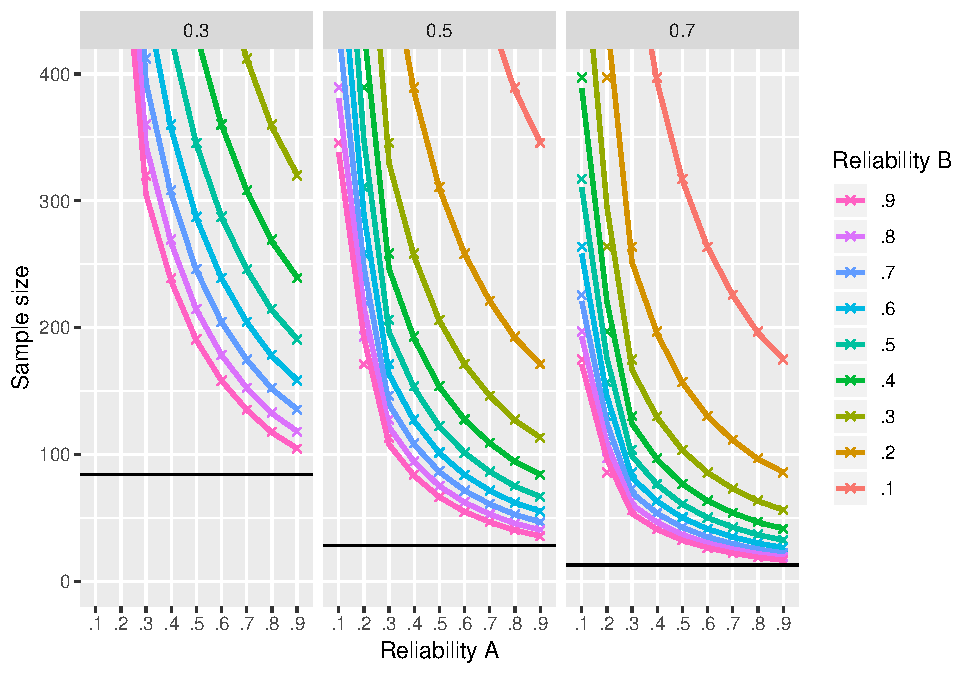
\includegraphics{Parsons_Kruijt_Fox_-_reporting_reliability_files/figure-latex/figuretwo-1.pdf}
\caption{\label{fig:figuretwo}Required sample size for 80\% power to detect \enquote{true} correlations of .3, .5, and .7 that have been corrected for reliability of measure A and B. The horizontal lines indicate the sample size required assuming perfect reliability of measures A and B.}
\end{figure}

For those interested in applying multi level modelling: two recent papers have explored the use of hierarchical models to account for one source of error-variance, namely trial-level variation (J. Rouder \& Haaf, 2018a; Rouder et al., 2019). The authors demonstrate that Spearman's correction formula for attenuation can be unstable and proposed it is outperformed by trial-level hierarchical models. However, none of the models tested in in Rouder, Kumar, and Haaf (2019) performed well enough to accurately recover the simulated effect size. This has been ascribed to the little true individual variation in the inhibition tasks explored by the authors. In other words, error-variance (measurement noise) may render true-variance relationship unrecoverable. In this paper we focus on estimating the reliability of measures, in part to assist correcting for measurement error -- though we advise readers to refer elsewhere for guidance on correcting estimates (e.g.~Rouder et al., 2019; Schmidt \& Hunter, 1996). In our experience multilevel models are not (yet) used as standard to analyse data from behavioural tasks, although we expect that they will become standard in the upcoming years. Nonetheless, this manuscript focusses on standard estimates of internal consistency and test-retest top help bridge the gap until they become the norm.

\hypertarget{reliability-and-comparability}{%
\subsection{Reliability and comparability}\label{reliability-and-comparability}}

Cooper and colleagues illustrate two potential pitfalls when comparing effect sizes without considering reliability, using data derived from the computerised \enquote{Continuous Performance Task} (the AX-CPT) as an example (Cooper et al., 2017). To illustrate a potential pitfall when comparing correlations between samples taken from different populations, they used AX-CPT data originally reported by Strauss et al., 2014 (including reliabilities for all their task measures). Cooper et al.~point out the observed higher correlations between the AX-CPT and another task measure (the Relational and Item-Specific Encoding task - RISE) in the schizophrenia sample compared to the control sample. It is discussed that the AX-CPT yielded greater variance in measure scores, and greater test-retest reliability across each trial type, in the schizophrenia sample compared to the control sample. Therefore, it cannot be ruled out that the differences in AX-CPT - RISE correlation between samples are the result of differences in variance and reliability between samples. Cooper et al.~next illustrate a potential pitfall when compared findings between largely identical studies, where one might expect results to replicate. For this demonstration, they used data from two studies examining the relationship between AX-CPT and working memory, each recruiting a separate sample of participants from the same population (Gonthier, Macnamara, Chow, Conway, \& Braver, 2016; Richmond, Redick, \& Braver, 2016). While the correlation between one AX-CPT trial type and working memory did replicate between studies, the correlations between two other AX-CPT trial types and working memory did not. Taken a step further, others have proposed that we should correct effect size estimates for measurement error by default, as arguably researchers are typically concerned with the relationships between actual traits or constructs instead of between measures of traits or constructs (Schmidt \& Hunter, 1996). Correcting for error would enable direct comparisons between the effect sizes Cooper et al.~report, for example. Thus, adopting a practice of reporting reliability as standard would allow for better generalisability of effect size estimates as well as accurate comparisons of effect sizes (including aggregation of effect sizes, as in meta-analyses).

\hypertarget{an-example-from-the-field-of-experimental-psychopathology---the-dot-probe-task}{%
\subsection{An example from the field of experimental psychopathology - The Dot-Probe task}\label{an-example-from-the-field-of-experimental-psychopathology---the-dot-probe-task}}

To build on the previous sections we discuss a specific example from the subfield of experimental psychopathology (for reviews, e.g.~Cisler \& Koster, 2010; Gotlib \& Joormann, 2010; Yiend, 2010). We focus on a task prolifically used to assess (and often, attempt to modify) selective attention bias; the emotional dot-probe task (MacLeod, Mathews, \& Tata, 1986). In a typical dot-probe task two stimuli are presented simultaneously for a set presentation duration (e.g.~500ms). Usually, one of the stimuli is emotional (e.g.~threat related), and the other is neutral. Immediately after the stimuli disappear, a probe is presented and participants make keyed responses based on the identity of the probe (e.g.~whether it is the letter \enquote{E} or \enquote{F}). The outcome measure is an attention bias index, calculated by subtracting the average response time trials in which probes appeared in the location of the emotional stimuli from the average reaction time for trials in which probes appeared in the location of the neutral stimuli. We stress that a large proportion of studies using the dot-probe adopt different variations of the task to address a wide variety of research questions. Any combination of the following may differ between two given dot-probe tasks; the number of trials, the stimuli presentation duration, the type of stimuli used (e.g.~words or images), the probes (and how easily they can be discerned, or even whether the task is to identify the probe or just the location of the probe), and the stimuli sets themselves.

The use of the dot-probe methodology has grown considerably over the last decade (Kruijt, Field, \& Fox, 2016, supplemental Figure 1) and the number of published studies now likely numbers in the thousands. This growth was in spite of two early papers highlighted reliability problems with the dot-probe (Schmukle, 2005; Staugaard, 2009). Where reliability estimates for the dot-probe task are reported, they tend to be unacceptably low (as low as -.12 in Waechter, Nelson, Wright, Hyatt, \& Oakman, 2014). It is important to note that the reported estimates range widely (Bar-Haim et al., 2010; Enock, Hofmann, \& McNally, 2014: r = -.23 to .70; also see Waechter \& Stolz, 2015). From 2014 onwards, there has been growing concern about the reliability of the task and several papers have directly examined it's psychometric properties (Brown et al., 2014; Kappenman, Farrens, Luck, \& Proudfit, 2014; Price et al., 2015; Sigurjónsdóttir, Sigurðardóttir, Björnsson, \& Kristjánsson, 2015; Waechter et al., 2014; Waechter \& Stolz, 2015). Alongside widespread calls to develop more reliable measures (e.g.~MacLeod \& Grafton, 2016; Price et al., 2015; Rodebaugh et al., 2016 ; Waechter \& Stolz, 2015) various recommendations have been made to improve the stability and reliability of the dot-probe task (e.g.~Price et al., 2015). Yet, a recent study found that a number of these recommendations did not lead to consistent improvements in reliability, and no version of the task (or data processing strategy) was found to have adequate reliability (Jones, Christiansen, \& Field, 2018).

Calls to improve the reliability of measures, and attempts to empirically test strategies to do so, are noble. Ultimately, however, the near absence of reliability reporting makes it impossible for us to even begin to guess how reliable our measurements are in the vast majority of studies. In a recent paper Rodebaugh and colleagues were able to identify only 13 studies that reported the reliability of the dot-probe (Rodebaugh et al., 2016). To our knowledge, it is still the case that if reliability estimates are reported it is in the context of papers focussing on the problem of low reliability, while papers assessing applied research questions very rarely report reliability estimates. This underlines two of our earlier points, a) that we cannot generalise a reliability estimate from one version of this task, in one sample, to another study, and b) as a result of substantially different levels of reliability it will be no trivial matter to make comparisons of results across dot-probe studies (Cooper et al., 2017). Thus, while the greatest problem in this area may be that the dot-probe task yields unreliable data, the more pressing barrier is the consistent omission to estimate and report the psychometrics of our measures in the first instance.

It is not our intention in this section to unduly attack the dot-probe task. We use this task, as an example from many candidates, to demonstrate how taking \enquote{psychometric free-reign} (Vasey et al., 2003, p. 84) with our measures is detrimental to cumulative science. Evidence continues to amount demonstrating the dangers of taking liberties with the psychometrics of our measures; poor reliability is detrimental to making sound inferences (Rodebaugh et al., 2016), psychometric information is commonly underreported (Barry, Chaney, Piazza-Gardner, \& Chavarria, 2014; Flake et al., 2017; Slaney, Tkatchouk, Gabriel, \& Maraun, 2009), and this lack of reporting may hide serious validity issues (Hussey \& Hughes, 2018). The purpose of this paper is not to quench any discussion or research by means of a generalised argument that our measures are not reliable, but rather to convince researchers that our field stands to benefit from improved psychometric reporting standards.

\hypertarget{questions-of-experimental-differences-and-of-individual-differences}{%
\subsection{Questions of experimental differences and of individual differences}\label{questions-of-experimental-differences-and-of-individual-differences}}

A distinction has been raised between experimental research (e.g.~group or manipulation differences) and individual differences research (e.g.~correlational) that is worth briefly discussing (e.g.~Cronbach, 1975, 1957; Borsboom, Kievit, Cervone, \& Hood, 2009). Experimental analyses thrive from a quality described as \enquote{precision} (e.g.~Luck, 2019), which is necessarily paired with low between-individual variance (De Schryver, Hughes, Rosseel, \& De Houwer, 2016), and this is perhaps reflected in a desire for more homogeneous groups (Hedge et al., 2018). However, low variance may a) be due to lack of sensitivity in a measure and b) low variance within a homogeneous group may result in difficulties rank-ordering participants within the group. Regardless the cause of low between-individuals (true) variance, when it's paired with any amount of error variance, this can easily result in low reliability. While it is clear that many tasks display robust between-group or between-condition differences, they also tend to have suboptimal reliability for individual differences research (Hedge et al., 2018). One such example is the Stroop task (Stroop, 1935). It has been asserted that the Stroop effect can be considered universal (i.e.~we can safely assume that everyone presents the stroop effect; MacLeod, 1991; J. Rouder \& Haaf, 2018b). Yet, the task does not demonstrate sufficient reliability for questions of individual differences (Hedge et al., 2018; Rouder et al., 2019). Thus, robust experimental effects should not be interpreted as an indication of high measure reliability or validity, nor does this provide sufficient information on the applicability of the measure for individual differences research (Cooper et al., 2017; Hedge et al., 2018). Unfortunately, it is common that tasks developed for experimental settings are used in individual differences research with little attention paid to their psychometric properties. As Rouder, Kumar, and Haaf (2019) recently demonstrated, the use of tasks that present low reliability in questions of individual differences is doomed to fail. Regardless of the research question and the analysis used, increased measurement error will be detrimental to the analysis and the inferences we can draw from it (e.g.~Kanyongo, Brook, Kyei-Blankson, \& Gocmen, 2007).

\hypertarget{barriers-to-a-standard-pratics-of-reporting-reliability}{%
\subsection{Barriers to a standard pratics of reporting reliability}\label{barriers-to-a-standard-pratics-of-reporting-reliability}}

We see two main barriers to implementing a standard practice of estimating and reporting reliability of cognitive-behavioural tasks. First, it may not be possible to estimate reliability for some measures in the first place. Perhaps the task or the data processing required is too complex, or perhaps another factor within the task, sample, context, or data collected leads to difficulties in estimating reliability. In cases such as these, the authors might consider stating that \enquote{to their knowledge, there is no appropriate procedure to estimate the reliability of this measure}. This would have the benefit of transparency. Further, a consideration of measure reliability in the absence of reliability estimates would also help in tempering interpretations of results, if only by pre-empting an implicit assumption that a measure is perfectly reliable and valid. Second, there is a lack of current practice, education, and -- in some instances -- the tools needed to implement a practice of estimating and reporting reliability for cognitive-behavioural measures. Psychometric training in core psychology is often limited to calculating Cronbach's alpha for self-report data; this, and similar, reliability estimates may not be applicable to cognitive-behavioural measures. If a suitable procedure to estimate reliability does not exist or is inaccessible, then it would be foolhardy to expect researchers to report reliability as standard practice. A similar argument has been made for the use of Bayesian statistics and sparked the development of JASP, a free open-source software similar to SPSS with the capacity to perform Bayesian analyses in an accessible way (Love et al., 2019; Marsman \& Wagenmakers, 2017; Wagenmakers et al., 2018). It is important to ensure that the tools required to estimate reliability are readily available and easily usable. Therefore, the second part of this paper forms a brief tutorial (with R code), with examples and recommendations, for estimating and reporting reliability.

\hypertarget{a-brief-introduction-to-a-few-methods-to-estimating-and-reporting-measurement-reliability}{%
\section{A brief introduction to (a few methods to) estimating and reporting measurement reliability}\label{a-brief-introduction-to-a-few-methods-to-estimating-and-reporting-measurement-reliability}}

In this section we outline approaches to estimate the reliability of one's task measurements, including; internal consistency and test-retest of task measurements. Figure 3 presents our core recommendations in flow-chart form. For each, we outline a recommended estimate, provide simple R code to acquire these estimates, and offer recommendations on reporting standards. First, we make some general considerations on estimating and reporting reliability.

\begin{figure}[h]

{\centering 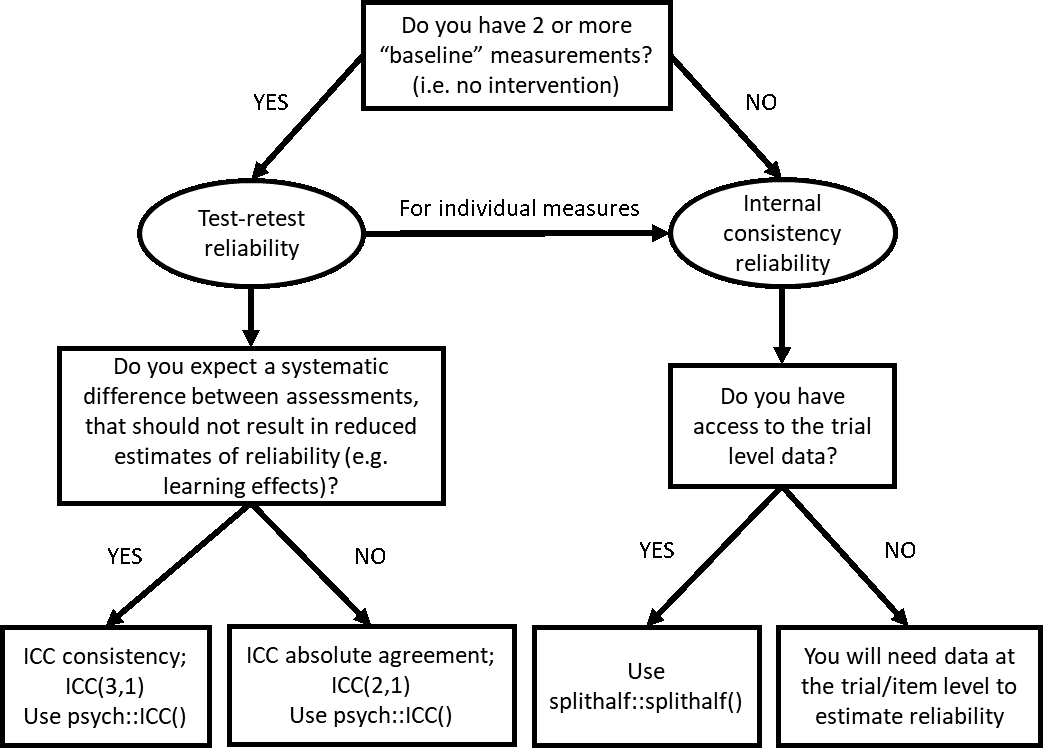
\includegraphics[width=0.8\linewidth]{fig3} 

}

\caption{Flowchart presentation of our core recommendations; report internal consistency reliability for individual measurements, and if multiple measurements are available also report test-retest reliability.}\label{fig:figthree}
\end{figure}

In this section we outline several approaches that can be taken to estimate the reliability of one's task measurements, including; internal consistency and test-retest of task measurements. For each, we outline the estimate, provide simple R code to acquire these estimates, and offer recommendations on reporting standards. First, some general considerations on estimating and reporting reliability.

\hypertarget{matching-reliability-and-outcome-scores}{%
\subsubsection{Matching reliability and outcome scores}\label{matching-reliability-and-outcome-scores}}

Reliability estimates should be drawn from the same data as the outcome scores. That is, if the outcome of interest entered into analysis is a difference score, the reliability of the difference score (and not it's components) should be determined. Likewise, removal of outlier trials, participants with high error rates, and so on, must be performed before reliability is estimated -- indeed, data reduction pipelines can have a surprising influence on reliability estimates. Likewise, if the data has been subset into several groups, it follows that reliability should be estimated for each group. Reliability should be estimated for the actual \emph{outcome measures to be analysed}.

\hypertarget{it-is-uninformative-to-report-p-values}{%
\subsubsection{It is uninformative to report p-values}\label{it-is-uninformative-to-report-p-values}}

We do not recommend that p-values are reported alongside reliability estimates. In our view it is often unclear what the p-value adds or indicates in this context, while it opens a potential misinterpretation that when an estimate differs significantly from zero one can be confidence in that reliability of that measurement. On several occasions we have observed statements describing measurement reliability as being statistically significant, albeit with low estimates (e.g.~\textless{} .3); avoiding this misunderstanding by simply not reporting p-values is preferable. Confidence intervals for reliability estimates, on the other hand, are informative and we recommend reporting them is more interpretable.

\hypertarget{thresholds-for-reliability}{%
\subsubsection{Thresholds for reliability}\label{thresholds-for-reliability}}

We refrain from making specific recommendations for what should be considered \enquote{adequate} or \enquote{excellent} reliability. Reliability estimates are continuous and using arbitrary thresholds may hinder their utility. Others have suggested suitable reliability from a threshold of .7, or .8; or use labels for specific intervals, such as; .50 - .75 to indicate \enquote{moderate reliability}, .75 - .90 to indicate good reliability, and above .90 indicate excellent reliability (Koo \& Li, 2016). These labels should not be considered thresholds to pass, but as another means to assess the validity of results based on these measures that rely on these measures (Rodebaugh et al., 2016).

\hypertarget{negative-reliability-estimates}{%
\subsubsection{Negative reliability estimates}\label{negative-reliability-estimates}}

It is also possible for reliability estimates to be negative. At first sight such a finding may indicate the (in many contexts mind-boggling) conclusion that those individuals who scored highest on the first test(half), scored lowest in the second and vice-versa. However, negative reliability estimates can spuriously arise for at least two reasons. This first is when the data violate the assumption of equal covariances among half-tests (Cronbach \& Hartmann, 1954). A second cause of spurious negative reliability estimates is specific for difference score outcomes (e.g.~bias indices or gain scores), and occurs when the correlation between the component scores is very high. When the components of a difference score correlate highly, the variance of the difference score will approach zero. At zero variance, reliability is also zero, but due to imprecision in the estimate, the correlation between two test-halfs or assessments may appear negative. In such cases, it appears as if the data has an impossible covariance structure with the total proportion of variance explained by the difference plus its component scores surpassing the maximum value of 1 (all variance observed). In cases where an unlikely negative reliability is obtained, we recommend to report the negative estimate as obtained, yet interpret it as equalling zero reliability (indeed, the value of 0 will typically be included in the estimate's confidence interval).

\hypertarget{report-the-complete-analysis}{%
\subsubsection{Report the complete analysis}\label{report-the-complete-analysis}}

Multiple approaches may be used to obtain the different estimates of reliability indicated by the same name. For example, using a split-half approach one could split trials into odd and even numbered trials, or alternatively, one could split trials into the first half and second half of trials. In addition to the reliability estimates themselves, we recommend authors report the analysis procedure used to obtain reliability estimates fully in order to facilitate transparency and reproducibility (providing analysis code would be ideal). These details would include; if and how data is subset, the reliability estimation method used, and the number of permutations or bootstraps if applicable. In addition, we recommend that confidence intervals are reported (e.g.~Koo \& Li, 2016) and note that reporting both corrected and uncorrected estimates (e.g.~in the case of splithalf reliability) can be useful to ease comparisons of estimates across studies.

\hypertarget{the-example-data}{%
\subsection{The example data}\label{the-example-data}}

For the following examples, we use Stroop task data from Hedge et al.~(2018). The data and code to recreate these analyses can be found in the Open Science Framework repository for this paper (\url{https://osf.io/9jp65/}). Briefly, in Hedge and colleagues' Stroop task, participants made keyed responses to the colour of a word presented centrally on-screen. In \enquote{congruent} trials the word was the same as the font colour. In \enquote{incongruent} trials, the word presented would be different from the font colour. Participants completed 240 trials of each trial type. For the purposes of this example we will focus on the RT cost outcome measure, calculated by subtracting the mean RT in congruent trials from the mean RT in incongruent trials. Participants completed the Stroop task twice, approximately three weeks apart. This is useful for our purposes as it allows us to investigate both; the internal consistency reliability of each measurement separately, as well as the test-retest reliability. Hedge et al.~report Stroop data from two separate studies; for simplicity, we have pooled this data. Data reduction follows the original paper and exact details can be found in the Rmarkdown version of this document (OSF repository: \url{https://osf.io/9jp65/}).

\hypertarget{internal-consistency-permutation-based-split-half-correlations}{%
\subsection{Internal consistency: Permutation-based split half correlations}\label{internal-consistency-permutation-based-split-half-correlations}}

Various statistical software programs offer the option to compute Cronbach's alpha, yet many of these use an approach that is unlikely to be suitable for cognitive-behavioural tasks. The most commonly used approach to estimate Cronbach's alpha amounts to averaging the correlations between each item score and the sum score of the remaining items. I.e. it assumes that item 1, item 2, item 3, etc etc. has been identical for all participants, It appears that in order to apply this approach to behavioural task data, researchers often resort to creating bins of trials, each to be treated as an individual \enquote{item} or mini-test. However, unless the task presents trial stimuli and conditions in a fixed order, Cronbach's alpha derived with this approach will not be a valid estimate of reliability. If we bin by trial number then the stimuli presented within each bin will differ between participants. In cases where the same set of trials (e.g.~same stimuli, etc.) have been offered in random order to the different participants, we could bin by stimuli (e.g.~by a specific pair of word content and colour in the Stroop example earlier), yet each bin/item-set will contain trials from different stages of the task which may reduce the obtained reliability estimate. We also note that while Omega has been advocated as a robust estimate to replace alpha (Dunn, Baguley, \& Brunsden, 2014; Peters, 2014; Sijtsma, 2009; Viladrich, Angulo-Brunet, \& Doval, 2017), the same assumption that each bin is equal across participants applies. Thus, the most common approach to obtaining alpha and omega is unsuitable for most task designs, except when a fixed trial and stimuli order was used.

However, the approach of obtaining alpha by averaging the correlation between each item and the sum of the other items, is only one way to approach to estimate alpha which is define as the average of all possible correlation between subsets of items. As such, it is also possible to approach alpha as average of a sufficiently large number of split-half reliability estimates (Spearman, 1910) when each split-half reliability is based on a different random division of the items.. In the split-half method as it is commonly applied, a measurement is split into two halves, typically by either the first vs the second half or by odd vs even numbered items or trials. The correlation between these halves is then calculated as an estimate of the internal reliability of a measure. The Spearman-Brown (prophecy) formula (Brown, 1910; Spearman, 1910) is often subsequently applied to this estimation. The correction accounts for the underestimation of reliability estimates resulting from splitting the number of observations in half to enable correlation. It is calculated as follows;

\begin{align}
r_s=\frac{2r}{1 + r}
\end{align}

Where \(r_s\) Spearman-Brown corrected estimate, and \emph{r} is the observed Pearson correlation between the two halves. When applied to tasks, standard split-half reliability estimates tend to be unstable. For example, reliability estimates obtained from splitting the data into odd and even numbered trials have the potential to vary greatly depending on which trials happen to be odd and even (Enock, Robinaugh, Reese, \& McNally, 2011). Therefore, Enock and colleagues estimated measurement reliability with a permutation approach. This process involves a large number of repeated calculations in which the data is randomly split into two halves and the reliability estimate is calculated (also see Cooper et al., 2017; MacLeod et al., 2010). The estimates are then averaged to provide a more stable estimate of reliability. It is important to note that Cronbach's alpha can be defined as the average of all possible split-half reliabilities (Cronbach, 1951). The permutation-based split-half reliability approach therefore approximates Cronbach's alpha, while being robust to the issues discussed above. We recommend that researchers estimate and report a permutation-based split-half estimate of internal consistency reliability.

The R package splithalf (Parsons, 2019); was developed to enable colleagues to apply this method to (trial level) task data with relative ease and minimal programming experience. Full documentation of the function, with examples, can be found online \url{https://sdparsons.github.io/splithalf_documentation/}. Please note that the online documentation will be the most up-to-date, and future package versions may use a different format to the one in this paper (version 0.5.2).

The permutation split-half approach can be performed on the Stroop data using the following code. The first line of code loads the splithalf package. The command \emph{splithalf}() calls the function, and contained within the parentheses are the function parameters. In this example we have specified that the data to be processed is contained within the object \enquote{Hedge\_raw}. We are interested in the response time cost, which is calculated as the difference between the mean RT in congruent trials and incongruent trials. Thus, we specify the outcome and score parameters as \enquote{difference} and \enquote{RT}, respectively. We also specify congruent and incongruent as the trial types that the difference score is calculated between. The parameters beginning in \enquote{var.} specify the variable name within the dataset and should be self-explanatory. Finally, we also specified in \enquote{conditionlist} that we would like the function to return separate estimates for the first and second testing session.

\begin{Shaded}
\begin{Highlighting}[]
\KeywordTok{require}\NormalTok{(splithalf)}
\KeywordTok{splithalf}\NormalTok{(}\DataTypeTok{data =}\NormalTok{ Hedge_raw,}
          \DataTypeTok{outcome =} \StringTok{"RT"}\NormalTok{,}
          \DataTypeTok{score =} \StringTok{"difference"}\NormalTok{,}
          \DataTypeTok{var.trialnum =} \StringTok{"Trial"}\NormalTok{,}
          \DataTypeTok{var.condition =} \StringTok{"time"}\NormalTok{,}
          \DataTypeTok{conditionlist =} \KeywordTok{c}\NormalTok{(}\DecValTok{1}\NormalTok{, }\DecValTok{2}\NormalTok{),}
          \DataTypeTok{var.compare =} \StringTok{"Condition"}\NormalTok{,}
          \DataTypeTok{compare1 =} \StringTok{"congruent"}\NormalTok{,}
          \DataTypeTok{compare2 =} \StringTok{"incongruent"}\NormalTok{,}
          \DataTypeTok{var.participant =} \StringTok{"ppid"}\NormalTok{,}
          \DataTypeTok{var.RT =} \StringTok{"Reactiontime"}\NormalTok{ )}
\end{Highlighting}
\end{Shaded}

Running this code will produce the following output. Note that estimates may differ slightly as a result of the permutation approach, but these differences will rarely exceed .01 with the default 5000 random splits. More splits will yield more precise estimates, but come at the expense of processing time; we recommend 5000 as the minimum.

\begin{verbatim}
  condition   n splithalf 95_low 95_high spearmanbrown SB_low SB_high
1         1 107      0.51   0.41    0.61          0.68   0.58    0.76
2         2 107      0.46   0.35    0.57          0.63   0.52    0.73
\end{verbatim}

The output includes two rows, in this case one for each testing session (the \enquote{condition} column). The \enquote{n} column provides a useful check that the expected number of participants have been processed. \enquote{splithalf} provides the average splithalf reliability estimate, and \enquote{spearmanbrown} provides the Spearman-Brown corrected estimate. The remaining columns provide the lower and upper 95\% percentile intervals for both the splithalf and the Spearman-Brown corrected estimate. The output might be reported as follows;

\emph{Permutation-based split-half reliability estimates were obtained, separately for each time-point using the splithalf package (version 0.5.2; Parsons, 2019) averaging the results of 5000 random splits. Reliability estimates were; time 1: r = 0.51, 95\%CI {[}0.41,0.61{]} (Spearman-Brown corrected estimates were r\textsubscript{SB} = 0.68, 95\%CI {[}0.58,0.76{]}), time 2: r = 0.46, 95\%CI {[}0.35,0.57{]} (Spearman-Brown corrected estimates were r\textsubscript{SB} = 0.63, 95\%CI {[}0.52,0.73{]}).}

\hypertarget{test-retest-intraclass-correlation-coefficients}{%
\subsection{Test-retest: IntraClass Correlation coefficients}\label{test-retest-intraclass-correlation-coefficients}}

While the random-splits splithalf method, delineated above, provides an estimate of the stability of a measures outcome within a single assessment, test-retest reliability provides an indication of the stability of a measure's scores over time. The timeframe for the re-test is an important consideration in the interpretation of test-retest estimates. For example, consider the difference in (intuitive) interpretation between test-retest reliability assessed over an one hour period versus a much longer period, e.g.~one-year. These variations of test-retest reliability have been described as indexing dependability and stability, respectively (Hussey \& Hughes, 2018; Revelle, 2017) - although the exact timings that constitute either descriptions are not agreed upon. Thus, for the interpretation of a test-retest estimate, it is important to consider the extent to which one would expect the construct of interest to remain stable over the period of time elapsed between the two assessments. Arguments to take into account include the extent to which task performance is expected to vary as a result of random processes -- such as mood fluctuations -- and more systematic processes such as practice or diurnal effects. Most indices of test-retest reliability are not affected by systematic changes between assessments, provided that all participants are affected to the exact same extent (a notable exception are the ICC agreement estimates which we discuss below). Yet, in practice, systematic processes affecting performance impact individuals to various degrees, thereby reducing test-retest reliability. It follows that the extent to which low test-retest reliability should reduce our confidence in analytical results based on that measure will depend much on the study design and the assumed characteristics of the construct being measured. Low test-retest reliability might be considered more problematic for a trait construct, compared to a state construct, for instance. Indeed, even low estimates of internal reliability may be theorized to be due to the construct fluctuating so rapidly that it cannot be measured reliably. Yet when a construct by its very nature cannot be measured reliably, it seems to follow that it then can also not be reliably studied or even verified to exist.

\hypertarget{estimating-reliability}{%
\subsubsection{Estimating reliability}\label{estimating-reliability}}

Test-retest reliability is often calculated as the Pearson correlation between two assessments of the same measure taken from the same sample. The summary data provided by Hedge et al.~was collated into a single data frame \enquote{summary} and for simplicity we shortened the variable names to \enquote{Stroop\_1} and \enquote{Stroop\_2}. This is easily performed in R. From a plethora of correlation functions available in R, we opted to use the function \emph{cor.test}() because it is part of the stats package that is installed by default, and because it also returns the 95\% Confidence Interval for the point estimate.

\newpage

\begin{Shaded}
\begin{Highlighting}[]
\KeywordTok{cor.test}\NormalTok{(summary}\OperatorTok{$}\NormalTok{Stroop_}\DecValTok{1}\NormalTok{, summary}\OperatorTok{$}\NormalTok{Stroop_}\DecValTok{2}\NormalTok{)}
\end{Highlighting}
\end{Shaded}

\begin{verbatim}

    Pearson's product-moment correlation

data:  summary$Stroop_1 and summary$Stroop_2
t = 10.567, df = 98, p-value < 2.2e-16
alternative hypothesis: true correlation is not equal to 0
95 percent confidence interval:
 0.6225912 0.8100704
sample estimates:
      cor 
0.7297674 
\end{verbatim}

Thus, from the output we observe a test-retest reliability of r = 0.73, 95\% CI {[}0.62 - 0.81{]}. Pearson's correlation provides an easily obtained indication of the consistency between the two measurements, the value of which tends to be close to the value that would be obtained if the data was analysed more extensively using a method called variance decomposition. In variance decomposition, which is closely related to analysis of variance, the variance on the outcome measure is divided into true variance (within and/or between) and error variance which can then be used to calculate test-retest reliability as true variance / true variance + error variance. Correlation estimates obtained through variance decomposition are named IntraClass Correlation (ICC), and were first introduced by Fisher (1954). An ICC taking into account only the decomposition in true and error variance reflects what is called consistency, i.e.~the extent to which the individuals are ranked in the same order/pattern between the two assessments. However, it has been argued that test-retest reliability should reflect agreement, rather than consistency, between measurements (2016). For example, a perfect correlation between scores at two time points may occur also when there is a systematic difference between time points (i.e.~a difference that is about equal for all participants. For a measure that has a pre-defined boundary value this may mean that despite perfect consistency, some or all participants may be classified differently between the two assessments dependent on whether their score ended up on one or the other side of the boundary value. Imagine a scenario in which we have two measurements and the second is simply the first measurement plus a fixed amount, e.g.~all participants improved by 10 on our fictional measure. This change may be a result of practice effects, development, or perhaps some other systematic difference over time. It is up to the researcher to determine the importance -- and relevance to the research question -- of these kinds of potential systematic changes in scores, and use this decision to guide the decision of which ICC approach is most applicable. In this case the consistency (and the correlation) would be extremely high, whereas the absolute agreement would be lower as the difference between sessions is taken into account.

In practice, there exists a multitude of ICC approaches. There are ten variations of the ICC described by McGraw and Wong (1996) and six described by Shrout and Fleiss (1979). Each set of authors with their own conventions for describing the variations. In part due to these differences in conventions it can be difficult to determine which variation is most appropriate. Helpfully, Koo and Li (2016) provide a comparison of conventions, and the relevant formulas. For the purposes of cognitive-behavioural tasks, there are two ICC variations most appropriate; ICC(2,1) and ICC(3,1) in the Shrout and Fleiss convention - these correspond to agreement and consistency, respectively. Both are based on variance decomposition using a two-way mixed-effects model of the single rater type. The primary decision for researchers is whether they are primarily concerned with the consistency (ICC3,1) or the absolute agreement (ICC2,1) of their measures as described above -- though we suggest that reporting both estimates is valuable as it allows for a comparison between consistency and agreement of the measures. To illustrate the distinction beteen ICC estimates, we present the equations for each ICC below (simplified from Koo \& Li, 2016). For simplicity, \enquote{between} refers to between-subjects variance, \enquote{within} refers to within-subjects or between-sessions variance, and \enquote{error} refers to error variance; finally, \enquote{k} is the number of measurements, and \enquote{n} is the sample size. Note that agreement (equation 6) extends consistency (equation 5) by including within-subjects variance (changes between tests) in the denominator. This causes the denominator to be larger if there is error associated with differences between sessions within participants, resulting in lower ICC estimates for agreement compared to consistency.

\begin{align}
ICC(3,1) consistency=\frac{between - error}{between + (k-1)error}
\end{align}

\begin{align}
ICC(2,1) agreement=\frac{between - error}{between + (k-1)error + \frac{k}{n}(within - error)}
\end{align}

Helpfully, ICCs (including 95\% confidence intervals) can be estimated easily in R using the psych package (Revelle, 2017). In the code below we first load the psych package before calling the ICC function. We select data from the two available time points; \enquote{Stroop\_1}, and \enquote{Stroop\_2}. The standard output includes six variations of the ICC and related test statistics (note we have altered the output slightly to be more presentable in this paper).

\begin{Shaded}
\begin{Highlighting}[]
\KeywordTok{require}\NormalTok{(psych)}
\KeywordTok{ICC}\NormalTok{(}\KeywordTok{select}\NormalTok{(summary, Stroop_}\DecValTok{1}\NormalTok{, Stroop_}\DecValTok{2}\NormalTok{))}
\end{Highlighting}
\end{Shaded}

\begin{verbatim}
   type  ICC    F df1 df2      p lower bound upper bound
1  ICC1 0.62 4.25  99 100 < .001        0.48        0.73
2  ICC2 0.64 6.19  99  99 < .001        0.31        0.80
3  ICC3 0.72 6.19  99  99 < .001        0.61        0.80
4 ICC1k 0.76 4.25  99 100 < .001        0.65        0.84
5 ICC2k 0.78 6.19  99  99 < .001        0.47        0.89
6 ICC3k 0.84 6.19  99  99 < .001        0.76        0.89
\end{verbatim}

We are interested in the second and the third rows of the output, corresponding to the ICC2 (absolute agreement) and ICC3 (consistency). Researchers may be more interested in one estimate over another due to any of the reasons we discussed above, though reporting both would provide a more comprehensive picture of the measure's reliability. The ICC column is our test-retest reliability estimate, and the final two columns are the lower and upper 95\% confidence intervals around the point estimate. The ICC estimate might be reported as follows;

Test-retest reliability for the Stroop task between the first and second testing session was estimated using Intraclass Correlation Coefficient (ICC; and accompanying 95\% confidence intervals) using the psych package in R (Revelle, 2017). We report two-way mixed effects models for absolute agreement, ICC(2,1), and consistency, ICC(3,1). The estimated agreement ICC(2,1) was, ICC = 0.64, 95\% CI {[}0.31, 0.80{]}, and the estimated consistency was, ICC = 0.72, 95\% CI {[}0.61, 0.80{]}.

\hypertarget{extensions-of-the-icc-approach}{%
\subsubsection{Extensions of the ICC approach}\label{extensions-of-the-icc-approach}}

Two additional indices may be drawn from the ICC to be used to assist researchers in their interpretations, both of which are discussed in detail by Hedge et al.~(2018). The first involves examining the relative variances contributed by within-subjects, between-subjects, and error variances. The ICC enables researchers to examine these relative proportions of total variance. This is useful, as a single index of reliability cannot convey all of the important information that a researcher may be interested in. The relative variances may also be helpful to give an impression of where variance may be \enquote{spent} on our analyses. The second involves reporting the standard error of measurement which can be calculated as the square root of error variance in the ICC calculation to reflect the 68\% confidence interval for scores observed on the task. This can provide a useful indication of the degree of measurement error on individual scores as it is in the same scale as the original score. Though, the size of the SEM is perhaps less easy to apply than reliability estimates. For example, is a 20ms SEM, or a 50ms SEM, acceptable in the current paradigm? While this is an unsolved problem, reporting standard error of measurement alongside our estimates of reliability may provide further useful information to guide the interpretation of results. For instance, Hedge et al.~(2018) note both small SEM and low reliability in their Flanker task measurements. The low SEM suggests that participants perform in a relatively similar way across sessions; yet, the low reliability suggests that participants are not similarly ranked across sessions. To ease the estimation of the relative variance, and standard error of measurement, we provide some code to extract the relative proportions of variance explained and the standard error of measurement adapted from the ICC function in the psych R package (Revelle, 2017). The code can be found in the markdown version of this paper in the OSF repository (\url{https://osf.io/9jp65/}). The code can be called with the function ICCdecompose;

\begin{Shaded}
\begin{Highlighting}[]
\KeywordTok{ICCdecompose}\NormalTok{(}\KeywordTok{select}\NormalTok{(summary, Stroop_}\DecValTok{1}\NormalTok{, Stroop_}\DecValTok{2}\NormalTok{))}
\end{Highlighting}
\end{Shaded}

\begin{verbatim}
  ICC21 lower upper   SEM BS_relative ERR_relative WS_relative
1  0.64  0.31   0.8 22.88        0.64         0.25        0.11
\end{verbatim}

The function returns the ICC(2,1) estimate, with lower and upper 95\% confidence intervals. Also returned are the SEM, and the relative proportions of variance explained by between-subjects (BS\_relative), error (ERR\_relative), and within-subjects (WS\_relative) variances.

\hypertarget{other-recommendations}{%
\subsubsection{Other recommendations}\label{other-recommendations}}

The chief aim of this paper is to argue for a culture change and to encourage researchers to adopt a standard practice of estimating and reporting the reliability of their measurements. There are two other related recommendations we would like to make. First, while most of our recommendations are aimed at researchers in examining the psychometrics of their own tasks, it is also the responsibility of journal editors and peer-reviewers to request psychometric information on cognitive and behavioural assessment tasks, just as they would for questionnaire measures. Similar to enforcing that authors report effect sizes and confidence intervals, or precise p values, reviewers could consider requesting psychometric evaluation of all measures used, whether they are based on self-report or other behavioural data. Indeed, reporting the psychometric properties of measurements falls clearly within APA reporting standards (Appelbaum et al., 2018, p. 7). Second, to fill the current gap in our knowledge on task reliability, we recommend that when developing novel computerised tasks (or adapting existing ones) researchers conduct validation studies for the new measures, including reporting reliability. Another possibility would be to pool data from a number of (previously published) studies to perform a meta-analytic validation. These validation studies would also be valuable in the development of reliable and valid measurements, and work such as this should be encouraged. Providing open data would further assist researchers in examining the reliability of cognitive measures where reliability is unreported.

\hypertarget{summary}{%
\section{Summary}\label{summary}}

We have argued that researchers using cognitive behavioural measures should adopt a standard practice of estimating and reporting the reliability of these behavioural measures. We have discussed several issues that arise when an assessment measure has low reliability, difficulties in comparing effect size estimates when reliability is unknown, and pointed out the fact that reliability is so seldom reported that we cannot know the impact of these issues on the state of our knowledge. Beyond arguing that we need to report reliability estimates as standard, we sought to help make this a reality by providing some assistance to other researchers, in the form of a short tutorial and R code. Future researchers, especially those seeking to use a measure that has only been tested in experimental setting in their own correlational research, will benefit if reporting reliability becomes standard. We have an obligation to future researchers to provide a sound evidence base, and this includes developing valid and reliable tools. For this, we must develop a research culture that routinely estimates and reports measurement reliability for cognitive behavioural assessments.

\newpage

\hypertarget{references}{%
\section{References}\label{references}}

\setlength{\parindent}{-0.5in}
\setlength{\leftskip}{0.5in}
\setlength{\parskip}{8pt}

\noindent

\hypertarget{refs}{}
\leavevmode\hypertarget{ref-appelbaum_journal_2018}{}%
Appelbaum, M., Cooper, H., Kline, R. B., Mayo-Wilson, E., Nezu, A. M., \& Rao, S. M. (2018). Journal article reporting standards for quantitative research in psychology: The APA publications and communications board task force report. \emph{American Psychologist}, \emph{73}(1), 3--25. doi:\href{https://doi.org/10.1037/amp0000191}{10.1037/amp0000191}

\leavevmode\hypertarget{ref-R-papaja}{}%
Aust, F., \& Barth, M. (2018). \emph{papaja: Create APA manuscripts with R Markdown}. Retrieved from \url{https://github.com/crsh/papaja}

\leavevmode\hypertarget{ref-bar-haim_life-threatening_2010}{}%
Bar-Haim, Y., Holoshitz, Y., Eldar, S., Frenkel, T. I., Muller, D., Charney, D. S., \ldots{} Wald, I. (2010). Life-threatening danger and suppression of attention bias to threat. \emph{American Journal of Psychiatry}, \emph{167}(6), 694--698. doi:\href{https://doi.org/10.1176/appi.ajp.2009.09070956}{10.1176/appi.ajp.2009.09070956}

\leavevmode\hypertarget{ref-barry_validity_2014}{}%
Barry, A. E., Chaney, B., Piazza-Gardner, A. K., \& Chavarria, E. A. (2014). Validity and reliability reporting practices in the field of health education and behavior: A review of seven journals. \emph{Health Education \& Behavior}, \emph{41}(1), 12--18. doi:\href{https://doi.org/10.1177/1090198113483139}{10.1177/1090198113483139}

\leavevmode\hypertarget{ref-valsiner_two_2009}{}%
Borsboom, D., Kievit, R. A., Cervone, D., \& Hood, S. B. (2009). The two disciplines of scientific psychology, or: The disunity of psychology as a working hypothesis. In J. Valsiner, P. C. M. Molenaar, M. C. Lyra, \& N. Chaudhary (Eds.), \emph{Dynamic process methodology in the social and developmental sciences} (pp. 67--97). New York, NY: Springer US. doi:\href{https://doi.org/10.1007/978-0-387-95922-1_4}{10.1007/978-0-387-95922-1\_4}

\leavevmode\hypertarget{ref-brown_psychometric_2014}{}%
Brown, H., Eley, T., Broeren, S., MacLeod, C., Rinck, M., Hadwin, J., \& Lester, K. (2014). Psychometric properties of reaction time based experimental paradigms measuring anxiety-related information-processing biases in children. \emph{Journal of Anxiety Disorders}, \emph{28}(1), 97--107. doi:\href{https://doi.org/10.1016/j.janxdis.2013.11.004}{10.1016/j.janxdis.2013.11.004}

\leavevmode\hypertarget{ref-brown_experimental_1910}{}%
Brown, W. (1910). Some experimental results in the correlation mental health abilities. \emph{British Journal of Psychology, 1904-1920}, \emph{3}(3), 296--322. doi:\href{https://doi.org/10.1111/j.2044-8295.1910.tb00207.x}{10.1111/j.2044-8295.1910.tb00207.x}

\leavevmode\hypertarget{ref-button_social_2013}{}%
Button, K., Lewis, G., Penton-Voak, I., \& Munafò, M. (2013). Social anxiety is associated with general but not specific biases in emotion recognition. \emph{Psychiatry Research}, \emph{210}(1), 199--207. doi:\href{https://doi.org/10.1016/j.psychres.2013.06.005}{10.1016/j.psychres.2013.06.005}

\leavevmode\hypertarget{ref-R-pwr}{}%
Champely, S. (2018). \emph{Pwr: Basic functions for power analysis}. Retrieved from \url{https://CRAN.R-project.org/package=pwr}

\leavevmode\hypertarget{ref-cisler_mechanisms_2010}{}%
Cisler, J. M., \& Koster, E. H. (2010). Mechanisms of attentional biases towards threat in anxiety disorders: An integrative review. \emph{Clinical Psychology Review}, \emph{30}(2), 203--216. doi:\href{https://doi.org/10.1016/j.cpr.2009.11.003}{10.1016/j.cpr.2009.11.003}

\leavevmode\hypertarget{ref-cooper_role_2017}{}%
Cooper, S. R., Gonthier, C., Barch, D. M., \& Braver, T. S. (2017). The role of psychometrics in individual differences research in cognition: A case study of the AX-CPT. \emph{Frontiers in Psychology}, \emph{8}. doi:\href{https://doi.org/10.3389/fpsyg.2017.01482}{10.3389/fpsyg.2017.01482}

\leavevmode\hypertarget{ref-cronbach_l._j._coefficient_1951}{}%
Cronbach, L. J. (1951). Coefficient alpha and the internal structure of tests, \emph{16}(3), 297--334.

\leavevmode\hypertarget{ref-cronbach_two_1957}{}%
Cronbach, L. J. (1957). The two disciplines of scientific psychology. \emph{The Americal Psychologist}, \emph{12}(11), 671--684.

\leavevmode\hypertarget{ref-cronbach_beyond_1975}{}%
Cronbach, L. J. (1975). Beyond the two disciplines of scientific psychology. \emph{American Psychologist}, \emph{30}(2), 116--127. doi:\href{https://doi.org/10.1037/h0076829}{10.1037/h0076829}

\leavevmode\hypertarget{ref-cronbach_note_1954}{}%
Cronbach, L. J., \& Hartmann, W. (1954). A note on negative reliabilities. \emph{Educational and Psychological Measurement}, \emph{14}(2), 342--346. doi:\href{https://doi.org/10.1177/001316445401400213}{10.1177/001316445401400213}

\leavevmode\hypertarget{ref-de_schryver_unreliable_2016}{}%
De Schryver, M., Hughes, S., Rosseel, Y., \& De Houwer, J. (2016). Unreliable yet still replicable: A comment on LeBel and paunonen (2011). \emph{Frontiers in Psychology}, \emph{6}. doi:\href{https://doi.org/10.3389/fpsyg.2015.02039}{10.3389/fpsyg.2015.02039}

\leavevmode\hypertarget{ref-dunn_alpha_2014}{}%
Dunn, T. J., Baguley, T., \& Brunsden, V. (2014). From alpha to omega: A practical solution to the pervasive problem of internal consistency estimation. \emph{British Journal of Psychology}, \emph{105}(3), 399--412. doi:\href{https://doi.org/10.1111/bjop.12046}{10.1111/bjop.12046}

\leavevmode\hypertarget{ref-enock_attention_2014}{}%
Enock, P. M., Hofmann, S. G., \& McNally, R. J. (2014). Attention bias modification training via smartphone to reduce social anxiety: A randomized, controlled multi-session experiment. \emph{Cognitive Therapy and Research}, \emph{38}(2), 200--216. doi:\href{https://doi.org/10.1007/s10608-014-9606-z}{10.1007/s10608-014-9606-z}

\leavevmode\hypertarget{ref-enock_improved_2011}{}%
Enock, P. M., Robinaugh, D. J., Reese, H. E., \& McNally, R. J. (2011). Improved reliability estimation and psychometrics of the dot-probe paradigm on smartphones and PC (poster).

\leavevmode\hypertarget{ref-fisher_statistical_1954}{}%
Fisher, R. (1954). \emph{Statistical methods for research workers}. Oliver; Boyd.

\leavevmode\hypertarget{ref-flake_construct_2017}{}%
Flake, J. K., Pek, J., \& Hehman, E. (2017). Construct validation in social and personality research: Current practice and recommendations. \emph{Social Psychological and Personality Science}, \emph{8}(4), 370--378. doi:\href{https://doi.org/10.1177/1948550617693063}{10.1177/1948550617693063}

\leavevmode\hypertarget{ref-gawronski_response_2011}{}%
Gawronski, B., Deutsch, R., \& Banse, R. (2011). Response interference tasks as indirect measures of automatic associations. In \emph{Cognitive methods in social psychology} (pp. 78--123). New York, NY, US: The Guilford Press.

\leavevmode\hypertarget{ref-gonthier_inducing_2016}{}%
Gonthier, C., Macnamara, B. N., Chow, M., Conway, A. R. A., \& Braver, T. S. (2016). Inducing proactive control shifts in the AX-CPT. \emph{Frontiers in Psychology}, \emph{7}. doi:\href{https://doi.org/10.3389/fpsyg.2016.01822}{10.3389/fpsyg.2016.01822}

\leavevmode\hypertarget{ref-gotlib_cognition_2010}{}%
Gotlib, I. H., \& Joormann, J. (2010). Cognition and depression: Current status and future directions. \emph{Annual Review of Clinical Psychology}, \emph{6}(1), 285--312. doi:\href{https://doi.org/10.1146/annurev.clinpsy.121208.131305}{10.1146/annurev.clinpsy.121208.131305}

\leavevmode\hypertarget{ref-hedge_reliability_2018}{}%
Hedge, C., Powell, G., \& Sumner, P. (2018). The reliability paradox: Why robust cognitive tasks do not produce reliable individual differences. \emph{Behavior Research Methods}, \emph{50}(3), 1166--1186. doi:\href{https://doi.org/10.3758/s13428-017-0935-1}{10.3758/s13428-017-0935-1}

\leavevmode\hypertarget{ref-R-purrr}{}%
Henry, L., \& Wickham, H. (2019). \emph{Purrr: Functional programming tools}. Retrieved from \url{https://CRAN.R-project.org/package=purrr}

\leavevmode\hypertarget{ref-hussey_hidden_2018}{}%
Hussey, I., \& Hughes, S. (2018). Hidden invalidity among fifteen commonly used measures in social and personality psychology. doi:\href{https://doi.org/10.31234/osf.io/7rbfp}{10.31234/osf.io/7rbfp}

\leavevmode\hypertarget{ref-ioannidis_why_2005}{}%
Ioannidis, J. P. A. (2005). Why most published research findings are false. \emph{PLoS Medicine}, \emph{2}(8), 6.

\leavevmode\hypertarget{ref-ioannidis_false-positive_2011}{}%
Ioannidis, J. P. A., Tarone, R., \& McLaughlin, J. K. (2011). The false-positive to false-negative ratio in epidemiologic studies: \emph{Epidemiology}, \emph{22}(4), 450--456. doi:\href{https://doi.org/10.1097/EDE.0b013e31821b506e}{10.1097/EDE.0b013e31821b506e}

\leavevmode\hypertarget{ref-jones_failed_2018}{}%
Jones, A., Christiansen, P., \& Field, M. (2018). Failed attempts to improve the reliability of the alcohol visual probe task following empirical recommendations. \emph{Psychology of Addictive Behaviors}, \emph{32}(8), 922--932. doi:\href{https://doi.org/10.31234/osf.io/4zsbm}{10.31234/osf.io/4zsbm}

\leavevmode\hypertarget{ref-kanyongo_reliability_2007}{}%
Kanyongo, G. Y., Brook, G. P., Kyei-Blankson, L., \& Gocmen, G. (2007). Reliability and statistical power: How measurement fallibility affects power and required sample sizes for several parametric and nonparametric statistics. \emph{Journal of Modern Applied Statistical Methods}, \emph{6}(1), 81--90. doi:\href{https://doi.org/10.22237/jmasm/1177992480}{10.22237/jmasm/1177992480}

\leavevmode\hypertarget{ref-kappenman_behavioral_2014}{}%
Kappenman, E. S., Farrens, J. L., Luck, S. J., \& Proudfit, G. H. (2014). Behavioral and ERP measures of attentional bias to threat in the dot-probe task: Poor reliability and lack of correlation with anxiety. \emph{Frontiers in Psychology}, \emph{5}. doi:\href{https://doi.org/10.3389/fpsyg.2014.01368}{10.3389/fpsyg.2014.01368}

\leavevmode\hypertarget{ref-koo_guideline_2016}{}%
Koo, T. K., \& Li, M. Y. (2016). A guideline of selecting and reporting intraclass correlation coefficients for reliability research. \emph{Journal of Chiropractic Medicine}, \emph{15}(2), 155--163. doi:\href{https://doi.org/10.1016/j.jcm.2016.02.012}{10.1016/j.jcm.2016.02.012}

\leavevmode\hypertarget{ref-kruijt_capturing_2016}{}%
Kruijt, A.-W., Field, A. P., \& Fox, E. (2016). Capturing dynamics of biased attention: Are new attention variability measures the way forward? \emph{PLOS ONE}, \emph{11}(11), e0166600. doi:\href{https://doi.org/10.1371/journal.pone.0166600}{10.1371/journal.pone.0166600}

\leavevmode\hypertarget{ref-lebel_sexy_2011}{}%
LeBel, E. P., \& Paunonen, S. V. (2011). Sexy but often unreliable: The impact of unreliability on the replicability of experimental findings with implicit measures. \emph{Personality and Social Psychology Bulletin}, \emph{37}(4), 570--583. doi:\href{https://doi.org/10.1177/0146167211400619}{10.1177/0146167211400619}

\leavevmode\hypertarget{ref-love_jasp:_2019}{}%
Love, J., Selker, R., Marsman, M., Jamil, T., Dropmann, D., Verhagen, J., \ldots{} Wagenmakers, E.-J. (2019). JASP: Graphical statistical software for common statistical designs. \emph{Journal of Statistical Software}, \emph{88}(2). doi:\href{https://doi.org/10.18637/jss.v088.i02}{10.18637/jss.v088.i02}

\leavevmode\hypertarget{ref-luck_why_2019}{}%
Luck, S. J. (2019, February 19). \emph{Why experimentalists should ignore reliability and focus on precision}. Retrieved from \url{https://lucklab.ucdavis.edu/blog/2019/2/19/reliability-and-precision}

\leavevmode\hypertarget{ref-macleod_anxiety-linked_2016}{}%
MacLeod, C., \& Grafton, B. (2016). Anxiety-linked attentional bias and its modification: Illustrating the importance of distinguishing processes and procedures in experimental psychopathology research. \emph{Behaviour Research and Therapy}, \emph{86}, 68--86. doi:\href{https://doi.org/10.1016/j.brat.2016.07.005}{10.1016/j.brat.2016.07.005}

\leavevmode\hypertarget{ref-macleod_half_1991}{}%
MacLeod, C. M. (1991). Half a century of research on the stroop effect: An integrative review. \emph{Psychological Bulletin}, \emph{109}(2), 163--203.

\leavevmode\hypertarget{ref-macleod_attentional_1986}{}%
MacLeod, C., Mathews, A., \& Tata, P. (1986). Attentional bias in emotional disorders. \emph{Journal of Abnormal Psychology}, \emph{95}(1), 15--20.

\leavevmode\hypertarget{ref-macleod_appraising_2010}{}%
MacLeod, J. W., Lawrence, M. A., McConnell, M. M., Eskes, G. A., Klein, R. M., \& Shore, D. I. (2010). Appraising the ANT: Psychometric and theoretical considerations of the attention network test. \emph{Neuropsychology}, \emph{24}(5), 637--651. doi:\href{https://doi.org/10.1037/a0019803}{10.1037/a0019803}

\leavevmode\hypertarget{ref-marsman_bayesian_2017}{}%
Marsman, M., \& Wagenmakers, E.-J. (2017). Bayesian benefits with JASP. \emph{European Journal of Developmental Psychology}, \emph{14}(5), 545--555. doi:\href{https://doi.org/10.1080/17405629.2016.1259614}{10.1080/17405629.2016.1259614}

\leavevmode\hypertarget{ref-R-wordcountaddin}{}%
Marwick, B. (2019). \emph{Wordcountaddin: Word counts and readability statistics in r markdown documents}.

\leavevmode\hypertarget{ref-mcgraw_forming_1996}{}%
McGraw, K. O., \& Wong, S. P. (1996). Forming inferences about some intraclass correlation coefficients. \emph{Psychological Methods}, \emph{1}(1), 30--46.

\leavevmode\hypertarget{ref-R-koRpus}{}%
Michalke, M. (2018a). \emph{KoRpus: An r package for text analysis}. Retrieved from \url{https://reaktanz.de/?c=hacking\&s=koRpus}

\leavevmode\hypertarget{ref-R-sylly}{}%
Michalke, M. (2018b). \emph{Sylly: Hyphenation and syllable counting for text analysis}. Retrieved from \url{https://reaktanz.de/?c=hacking\&s=sylly}

\leavevmode\hypertarget{ref-R-koRpus.lang.en}{}%
Michalke, M. (2019). \emph{KoRpus.lang.en: Language support for 'koRpus' package: English}. Retrieved from \url{https://reaktanz.de/?c=hacking\&s=koRpus}

\leavevmode\hypertarget{ref-morey_why_2016}{}%
Morey, R. D., \& Lakens, D. (2016). Why most of psychology is statistically unfalsifiable, 32. Retrieved from\href{:\%20https://github.com/richarddmorey/psychology_resolution/\%20blob/master/paper/response.pdf}{: https://github.com/richarddmorey/psychology\_resolution/ blob/master/paper/response.pdf}

\leavevmode\hypertarget{ref-R-tibble}{}%
Müller, K., \& Wickham, H. (2019). \emph{Tibble: Simple data frames}. Retrieved from \url{https://CRAN.R-project.org/package=tibble}

\leavevmode\hypertarget{ref-R-splithalf}{}%
Parsons, S. (2017). Splithalf; calculate task split half reliability estimates. Retrieved from \url{https://doi.org/10.6084/m9.figshare.5559175.v2}

\leavevmode\hypertarget{ref-parsons_splithalf:_2019}{}%
Parsons, S. (2019). \emph{Splithalf: Robust estimates of split half reliability}. Retrieved from \url{https://doi.org/10.6084/m9.figshare.5559175.v5}

\leavevmode\hypertarget{ref-peters_alpha_2014}{}%
Peters, G. J. Y. (2014). The alpha and the omega of scale reliability and validity: Why and how to abandon cronbach's alpha and the route towards more comprehensive assessment of scale quality. doi:\href{https://doi.org/10.31234/osf.io/h47fv}{10.31234/osf.io/h47fv}

\leavevmode\hypertarget{ref-price_empirical_2015}{}%
Price, R. B., Kuckertz, J. M., Siegle, G. J., Ladouceur, C. D., Silk, J. S., Ryan, N. D., \ldots{} Amir, N. (2015). Empirical recommendations for improving the stability of the dot-probe task in clinical research. \emph{Psychological Assessment}, \emph{27}(2), 365--376. doi:\href{https://doi.org/10.1037/pas0000036}{10.1037/pas0000036}

\leavevmode\hypertarget{ref-R-base}{}%
R Core Team. (2018). \emph{R: A language and environment for statistical computing}. Vienna, Austria: R Foundation for Statistical Computing. Retrieved from \url{https://www.R-project.org/}

\leavevmode\hypertarget{ref-revelle_w_psych:_2017}{}%
Revelle, W. (2017). \emph{Psych: Procedures for personality and psychological research}. Northwestern University, Evanston, Illinois, USA.

\leavevmode\hypertarget{ref-R-psych}{}%
Revelle, W. (2018). \emph{Psych: Procedures for psychological, psychometric, and personality research}. Evanston, Illinois: Northwestern University. Retrieved from \url{https://CRAN.R-project.org/package=psych}

\leavevmode\hypertarget{ref-richmond_remembering_2016}{}%
Richmond, L. L., Redick, T. S., \& Braver, T. S. (2016). Remembering to prepare: The benefits (and costs) of high working memory capacity. \emph{Journal of Experimental Psychology: Learning, Memory, and Cognition}, \emph{41}(6), 1764--1777. doi:\href{https://doi.org/10.1037/xlm0000122}{10.1037/xlm0000122}

\leavevmode\hypertarget{ref-rodebaugh_unreliability_2016}{}%
Rodebaugh, T. L., Scullin, R. B., Langer, J. K., Dixon, D. J., Huppert, J. D., Bernstein, A., \ldots{} Lenze, E. J. (2016). Unreliability as a threat to understanding psychopathology: The cautionary tale of attentional bias. \emph{Journal of Abnormal Psychology}, \emph{125}(6), 840--851. doi:\href{https://doi.org/10.1037/abn0000184}{10.1037/abn0000184}

\leavevmode\hypertarget{ref-rouder_psychometrics_2018}{}%
Rouder, J., \& Haaf, J. M. (2018a). A psychometrics of individual differences in experimental tasks. doi:\href{https://doi.org/10.31234/osf.io/f3h2k}{10.31234/osf.io/f3h2k}

\leavevmode\hypertarget{ref-rouder_power_2018}{}%
Rouder, J., \& Haaf, J. M. (2018b). Power, dominance, and constraint: A note on the appeal of different design traditions, 8.

\leavevmode\hypertarget{ref-rouder_why_2019}{}%
Rouder, J., Kumar, A., \& Haaf, J. M. (2019). Why most studies of individual differences with inhibition tasks are bound to fail. doi:\href{https://doi.org/10.31234/osf.io/3cjr5}{10.31234/osf.io/3cjr5}

\leavevmode\hypertarget{ref-schmidt_measurement_1996}{}%
Schmidt, F. L., \& Hunter, J. E. (1996). Measurement error in psychological research: Lessons from 26 research scenarios. \emph{Psychological Methods}, \emph{1}(2), 199--223.

\leavevmode\hypertarget{ref-schmukle_unreliability_2005}{}%
Schmukle, S. C. (2005). Unreliability of the dot probe task. \emph{European Journal of Personality}, \emph{19}(7), 595--605. doi:\href{https://doi.org/10.1002/per.554}{10.1002/per.554}

\leavevmode\hypertarget{ref-shrout_intraclass_1979}{}%
Shrout, P. E., \& Fleiss, J. L. (1979). Intraclass correlations: Uses in assessing rater reliability, \emph{86}(2), 420--428.

\leavevmode\hypertarget{ref-sigurjonsdottir_barking_2015}{}%
Sigurjónsdóttir, Ó., Sigurðardóttir, S., Björnsson, A. S., \& Kristjánsson, Á. (2015). Barking up the wrong tree in attentional bias modification? Comparing the sensitivity of four tasks to attentional biases. \emph{Journal of Behavior Therapy and Experimental Psychiatry}, \emph{48}, 9--16. doi:\href{https://doi.org/10.1016/j.jbtep.2015.01.005}{10.1016/j.jbtep.2015.01.005}

\leavevmode\hypertarget{ref-sijtsma_use_2009}{}%
Sijtsma, K. (2009). On the use, the misuse, and the very limited usefulness of cronbach's alpha. \emph{Psychometrika}, \emph{74}(1), 107--120. doi:\href{https://doi.org/10.1007/s11336-008-9101-0}{10.1007/s11336-008-9101-0}

\leavevmode\hypertarget{ref-slaney_psychometric_2009}{}%
Slaney, K. L., Tkatchouk, M., Gabriel, S. M., \& Maraun, M. D. (2009). Psychometric assessment and reporting practices: Incongruence between theory and practice. \emph{Journal of Psychoeducational Assessment}, \emph{27}(6), 465--476. doi:\href{https://doi.org/10.1177/0734282909335781}{10.1177/0734282909335781}

\leavevmode\hypertarget{ref-spearman_proof_1904}{}%
Spearman, C. (1904). The proof and measurement of association between two things. \emph{The American Journal of Psychology}, \emph{15}(1), 72. doi:\href{https://doi.org/10.2307/1412159}{10.2307/1412159}

\leavevmode\hypertarget{ref-spearman_correlation_1910}{}%
Spearman, C. (1910). CORRELATION CALCULATED FROM FAULTY DATA. \emph{British Journal of Psychology, 1904-1920}, \emph{3}(3), 271--295. doi:\href{https://doi.org/10.1111/j.2044-8295.1910.tb00206.x}{10.1111/j.2044-8295.1910.tb00206.x}

\leavevmode\hypertarget{ref-staugaard_reliability_2009}{}%
Staugaard, S. R. (2009). Reliability of two versions of the dot-probe task using photographic faces, 12.

\leavevmode\hypertarget{ref-stroop_studies_1935}{}%
Stroop, J. R. (1935). Studies of interference in serial verbal reactions. \emph{Journal of Experimental Psychology}, \emph{18}, 643--662.

\leavevmode\hypertarget{ref-vacha-haase_reliability_2002}{}%
Vacha-Haase, T., Henson, R. K., \& Caruso, J. C. (2002). Reliability generalization: Moving toward improved understanding and use of score reliability. \emph{Educational and Psychological Measurement}, \emph{62}(4), 562--569. doi:\href{https://doi.org/10.1177/0013164402062004002}{10.1177/0013164402062004002}

\leavevmode\hypertarget{ref-vasey_research_2003}{}%
Vasey, M. W., Dalgleish, T., \& Silverman, W. K. (2003). Research on information-processing factors in child and adolescent psychopathology: A critical commentary. \emph{Journal of Clinical Child \& Adolescent Psychology}, \emph{32}(1), 81--93. doi:\href{https://doi.org/10.1207/S15374424JCCP3201_08}{10.1207/S15374424JCCP3201\_08}

\leavevmode\hypertarget{ref-viladrich_viaje_2017}{}%
Viladrich, C., Angulo-Brunet, A., \& Doval, E. (2017). Un viaje alrededor de alfa y omega para estimar la fiabilidad de consistencia interna. \emph{Anales de Psicología}, \emph{33}(3), 755. doi:\href{https://doi.org/10.6018/analesps.33.3.268401}{10.6018/analesps.33.3.268401}

\leavevmode\hypertarget{ref-waechter_measuring_2014}{}%
Waechter, S., Nelson, A. L., Wright, C., Hyatt, A., \& Oakman, J. (2014). Measuring attentional bias to threat: Reliability of dot probe and eye movement indices. \emph{Cognitive Therapy and Research}, \emph{38}(3), 313--333. doi:\href{https://doi.org/10.1007/s10608-013-9588-2}{10.1007/s10608-013-9588-2}

\leavevmode\hypertarget{ref-waechter_trait_2015}{}%
Waechter, S., \& Stolz, J. A. (2015). Trait anxiety, state anxiety, and attentional bias to threat: Assessing the psychometric properties of response time measures. \emph{Cognitive Therapy and Research}, \emph{39}(4), 441--458. doi:\href{https://doi.org/10.1007/s10608-015-9670-z}{10.1007/s10608-015-9670-z}

\leavevmode\hypertarget{ref-wagenmakers_bayesian_2018-2}{}%
Wagenmakers, E.-J., Love, J., Marsman, M., Jamil, T., Ly, A., Verhagen, J., \ldots{} Morey, R. D. (2018). Bayesian inference for psychology. Part II: Example applications with JASP. \emph{Psychonomic Bulletin \& Review}, \emph{25}(1), 58--76. doi:\href{https://doi.org/10.3758/s13423-017-1323-7}{10.3758/s13423-017-1323-7}

\leavevmode\hypertarget{ref-R-ggplot2}{}%
Wickham, H. (2016). \emph{Ggplot2: Elegant graphics for data analysis}. Springer-Verlag New York. Retrieved from \url{https://ggplot2.tidyverse.org}

\leavevmode\hypertarget{ref-R-tidyverse}{}%
Wickham, H. (2017). \emph{Tidyverse: Easily install and load the 'tidyverse'}. Retrieved from \url{https://CRAN.R-project.org/package=tidyverse}

\leavevmode\hypertarget{ref-R-forcats}{}%
Wickham, H. (2019a). \emph{Forcats: Tools for working with categorical variables (factors)}. Retrieved from \url{https://CRAN.R-project.org/package=forcats}

\leavevmode\hypertarget{ref-R-stringr}{}%
Wickham, H. (2019b). \emph{Stringr: Simple, consistent wrappers for common string operations}. Retrieved from \url{https://CRAN.R-project.org/package=stringr}

\leavevmode\hypertarget{ref-R-dplyr}{}%
Wickham, H., François, R., Henry, L., \& Müller, K. (2019). \emph{Dplyr: A grammar of data manipulation}. Retrieved from \url{https://CRAN.R-project.org/package=dplyr}

\leavevmode\hypertarget{ref-R-tidyr}{}%
Wickham, H., \& Henry, L. (2019). \emph{Tidyr: Easily tidy data with 'spread()' and 'gather()' functions}. Retrieved from \url{https://CRAN.R-project.org/package=tidyr}

\leavevmode\hypertarget{ref-R-readr}{}%
Wickham, H., Hester, J., \& Francois, R. (2018). \emph{Readr: Read rectangular text data}. Retrieved from \url{https://CRAN.R-project.org/package=readr}

\leavevmode\hypertarget{ref-wilkinson_statistical_1999}{}%
Wilkinson, L. (1999). Statistical methods in psychology journals. \emph{American Psychologist}, 11.

\leavevmode\hypertarget{ref-R-formatR}{}%
Xie, Y. (2019). \emph{FormatR: Format r code automatically}. Retrieved from \url{https://CRAN.R-project.org/package=formatR}

\leavevmode\hypertarget{ref-R-tufte}{}%
Xie, Y., \& Allaire, J. (2019). \emph{Tufte: Tufte's styles for r markdown documents}. Retrieved from \url{https://CRAN.R-project.org/package=tufte}

\leavevmode\hypertarget{ref-yiend_effects_2010}{}%
Yiend, J. (2010). The effects of emotion on attention: A review of attentional processing of emotional information. \emph{Cognition \& Emotion}, \emph{24}(1), 3--47. doi:\href{https://doi.org/10.1080/02699930903205698}{10.1080/02699930903205698}

\leavevmode\hypertarget{ref-zimmerman_resolving_2015}{}%
Zimmerman, D. W., \& Zumbo, B. D. (2015). Resolving the issue of how reliability is related to statistical power: Adhering to mathematical definitions. \emph{Journal of Modern Applied Statistical Methods}, \emph{14}(2), 9--26. doi:\href{https://doi.org/10.22237/jmasm/1446350640}{10.22237/jmasm/1446350640}


\end{document}
